\documentclass[conference]{IEEEtran}
%\hyphenation{op-tical net-works semi-conduc-tor}
\usepackage[bibstyle=ieee, citestyle=numeric-comp]{biblatex}
\usepackage{graphicx}
\usepackage{amsmath}
\usepackage{listings}
\usepackage{caption}
\usepackage{subcaption}
\usepackage{csquotes}
\usepackage{float}
\usepackage{color}
\usepackage{gensymb}
\usepackage{multirow}
\usepackage{array}
\usepackage{mathtools}
\usepackage[thinlines]{easytable}
\DeclarePairedDelimiter{\abs}{\lvert}{\rvert}
\usepackage[toc,page]{appendix}
\usepackage{setspace}
\usepackage{biblatex}
\addbibresource{ref.bib}
\captionsetup[figure]{labelfont={bf},labelformat={default},labelsep=period,name={Fig.}}
\addbibresource{ref.bib}
\renewcommand\IEEEkeywordsname{Keywords}
\usepackage{diagbox}

\begin{document}

\title{ Automatic Detection of Suspicious Bangla Text\\ Using Logistic Regression}

\author{\IEEEauthorblockN{\textbf{Omar Sharif}}
\IEEEauthorblockA{Dept. of Computer Science \& Engineering\\
Chittagong University of Engineering and Technology\\
Chittagong-4349, Bangladesh\\
Email: omar.shaif1303@gmail.com}
\and
\IEEEauthorblockN{\textbf{Mohammed Moshiul Hoque}}
\IEEEauthorblockA{Professor, Department of CSE\\
Chittagong University of Engineering and Technology\\
Chittagong-4349, Bangladesh\\
Email: mmoshiulh@gmail.com}}


\maketitle

%%%%%%% Abstract and Keyword section %%%%%%%
%%%%%%%%%%%%%%%%%%%%%%%%%%%%%%%%%%%%%%%%%%%%
\begin{abstract}
Suspicious Bangla text detection is a text classification problem of classifying Bangla text into suspicious and non suspicious category. In this paper, we have implemented a system using logistic regression and also found out the performance of different statistical machine learning algorithm for detecting suspicious Bangla text. To the best of our knowledge, it is the very first work on detecting suspicious Bangla text so we have to develop a corpus containing suspicious Bangla text. This paper shows comparison of accuracy for different machine learning algorithm which will be helpful to others. The experimental result shows maximum accuracy of 92\% for logistic regression using 1500 training documents and 500 testing documents. The overall accuracy can be increased by increasing the number of text documents in the dataset and considering semantic relations between words of a sentence.  
\end{abstract}
\vspace{0.3cm}
\begin{IEEEkeywords}
 Suspicious Bangla text, Text classification, Text classification methods, Bangla language processing, Machine learning. 
\end{IEEEkeywords}

\IEEEpeerreviewmaketitle

%%%%%%%%%% Introduction %%%%%%%%%%%%%%%%%%%%
%%%%%%%%%%%%%%%%%%%%%%%%%%%%%%%%%%%%%%%%%%%%
\section{\textbf{Introduction}}
Text classification is the task of assigning a text document into a set of predefined classes in an intelligent manner. Because of the rapid growth of online information, text classification has become more challenging and more important as well. Digitization has changed
the way we process and analyze information. There is an exponential increase in online availability of information. From web pages to emails, science journals, ebooks, learning content, news and social media are all full of textual data. Text classification performs an essential role in various applications that deals with organizing, classifying, searching and concisely representing a significant amount of information. Detecting suspicious text is typically a text classification problem where we have to classify a text as suspicious and not suspicious. Suspicious text detection is a kind of system where suspicious texts are identified by the keywords used in the text body. As most of our communications are text based, if we able to predict either a text is suspicious or not suspicious it will be very helpful for our law enforcement agencies to find the perpetrator and stop terrorist event. As far we know, no system is developed for detecting suspicious Bangla text. But such system is required to predict criminal activities, reduce virtual social harassment in social media, mitigate national privacy threats and overall ensure our national security by detecting suspicious communications. 

In this work, our original purpose is to develop a framework for detecting suspicious Bangla texts. However, it is a relatively new problem for Bangla language which has not enough resources in this context. During implementation our main challenge was to develop a well furnished dataset for our system. It is very important for the research community regarding Bangla language to develop a system which can detect suspicious communications in Bangla.

%%%%%%%%%% Related Work %%%%%%%%%%%%%%%%%%%%
%%%%%%%%%%%%%%%%%%%%%%%%%%%%%%%%%%%%%%%%%%%%
\section{\textbf{Related Work}}
A number of significant researches have already done in text classification in English and other language. Major works of text classification are email classification, research paper categorization, detecting suspicious profiles etc.
But research on Bangla text classification is in preliminary stage still now. However some mentionable works have been done for Bangla language processing.
\vspace{0.2cm}

Hossain et al. describes Bengali document categorization based on word embedding and statistical learning approaches\cite{hossain2018automatic}. It categorizes document into nine predefined categories with mentionable accuracy. An Arabic text categorization system is developed using naive bayes in control environment dataset with good accuracy\cite{alsaleem2011automated}.
Krendzelak et al. describe a system which categorize text with machine learning and hierarchical structures by using tree based naive bayesian categorization process\cite{krendzelak2015text, chy2014bangla}. It performs with low accuracy due to training techniques and training feature extraction process.
\vspace{0.2cm}

S. Alami et al. describes about different techniques to detect suspicious profiles using text analysis within social media\cite{alami2015detecting}. A system for detecting suspicious email using enhanced feature selection is proposed but it has low accuracy because of not having enough dataset\cite{nizamani2013modeling}. Text categorization of Turkish language using SVM is proposed which achieved better accuracy but due to large feature dimensions time complexity is large\cite{kaya2012sentiment}. Better result can be obtained by using clustering based approach \cite{ismail2014bangla, ahmad2016bengali} but a lot of problem exist with cluster-based solution. In our work, a system is developed and trained with different machine learning algorithms and overall accuracy of this algorithms is measured over our dataset.\par
In this paper, we have applied naive bayes classifier\cite{yoo2015classification}, support vector machine\cite{wei2012text}, logistic regression\cite{sharma2015active}, k-nearest neighbor algorithms (KNN)\cite{harisinghaney2014text}, decision trees\cite{chavan2014survey} to detect suspicious Bangla text and also find out the accuracy of this algorithms.

%%%%%%%%% Methodology %%%%%%%%%%%%%%%%%%%%%%
%%%%%%%%%%%%%%%%%%%%%%%%%%%%%%%%%%%%%%%%%%%%
\section{\textbf{Suspicious Text Detector}}
The key objective of our project is to design a system that can classify suspicious and non-suspicious text. \textbf{Fig} \ref{fig:proposed_model} shows an abstract view of our suspicious text detector classifier.

\begin{figure}[h!]
\centering
  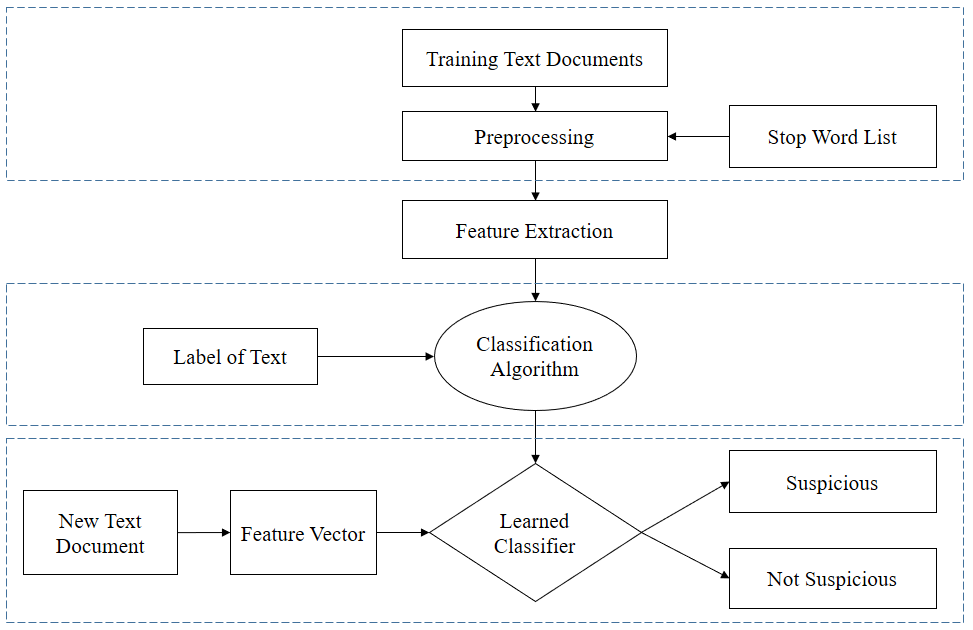
\includegraphics[height=6.8cm, width=8.8cm]{Figures/pr_model.PNG}
  \caption{ Model for Suspicious Text Detection}
  \label{fig:proposed_model}
\end{figure}

We have implemented this system by using different supervised machine learning algorithms. Our whole model is classified into four different phases.
\subsection{\textbf {Training Set Preparation}}
Our training set $T = \{t_1, t_2, t_3, ..., t_n\}$ is consist of $n$ training text documents. Each text is labeled as either suspicious or non suspicious. Suspicious class is denoted by $C_s$ and non suspicious class is denoted by $C_{ns}$.\par
A random text $t_i$ with $k$ words is represented by an one dimensional array $W[] =\{w_1, w_2, w_3, ....., w_k\}$ in our system,
\begin{table}[h!]
\begin{center}
\caption{Words of a Text}
\begin{tabular}{|m{1cm} | m{1cm}| m{1cm}|m{1cm} | m{1cm}|}
\hline
     $w_1$ & $w_2$  & $w_3$ & $...$ & $w_k$  \\
\hline
\end{tabular}
\end{center}
\end{table}

All texts are preprocessed by the preprocessor in order to remove inconsistencies for dataset. We have developed a list $S[]=\{s_1, s_2, s_3, ..., s_r\}$ with $r$ stopwords which is a column vector where each row contains a stop word.\par
\begin{table}[h!]
\begin{center}
\caption{Stop Word List}
\begin{tabular}{|m{0.7cm}|}
\hline
     $s_1$ \\
\hline
    $s_2$ \\
\hline 
    $s_3$ \\
\hline
 $...$ \\
 \hline
 $s_r$ \\
 \hline
\end{tabular}
\end{center}
\end{table}
\vspace{0.1cm}
In our system the word $w_i$ which has no contribution in deciding whether a text $t_i$ is suspicious ($C_s$) or not suspicious $(C_{ns})$ is referred as stop word $s_i$. Pronoun, conjunction, preposition, interjection, prefix and suffix are considered as stop words. Stop words $ s_1, s_2, s_3, ..., s_r$ are removed form the text $t_i$ by matching with a stop word list $S[]$. Punctuation's in a text are also removed in preprocessing step.


\subsection{\textbf{Feature Extraction}}
A word list is created by the tokenizer by tokenizing the main body of a text. Word frequencies is used as features in this system. Bag of words model is used to represent the features.
\renewcommand{\arraystretch}{1.3}
\begin{table}[h!]
\begin{center}
\caption{Feature Space}
\begin{tabular}{|m{0.7cm} | m{0.7cm}| m{0.7cm}|m{0.7cm} | m{0.7cm}|m{1cm}|m{0.7cm}|}
\hline
     & $w_1$ & $w_2$  & $w_3$ &$w_4$ &$...$ & $w_j$  \\
\hline
     $t_1$ & $2$ & $0$  & $0$ &$4$ &$...$ & $1$  \\
\hline
     $t_2$ & $0$ & $0$  & $1$ &$0$ &$...$ & $5$  \\
\hline
     $t_3$ & $4$ & $0$  & $2$ &$2$ &$...$ & $0$  \\
\hline
     $t_4$ & $0$ & $3$  & $0$ &$0$ &$...$ & $2$  \\
\hline
     $...$ & $...$ & ...  & $...$ &$...$ &$...$ & $...$  \\
\hline
     $t_i$ & $0$ & $0$  & $3$ &$1$ &$...$ & $0$  \\
\hline
\end{tabular}
\label{ff}
\end{center}
\end{table}
Table \ref{ff} shows the feature space for our system. Our feature space ($F[][]$) is a two dimensional ($i\times j$) array with $i$ rows and $j$ columns.
Here rows represents the texts $t_1, t_2, t_3, ..., t_i$ available in the corpus and columns represents total number unique words $w_1, w_2, w_3, ....., w_j$ in the corpus. Each cell of the array represents the frequency ($f_{ij}$) of a specific word $w_j$ occurs in a specific text $t_i$. Each row of the feature matrix represent features $F[][] =\{F[1], F[2], F[3], ... ,F[n]\} $ for the texts of the dataset. 

\subsection{\textbf{Classification Algorithm}}
It is most important part of our whole system. By using extracted features $F[1], F[2], F[3], ... ,F[n]$ and applying a suitable learning algorithm we train our model to classify texts as suspicious $C_s$ and non suspicious $C_{ns}$. Mainly logistic regression is used to implement the system and other algorithms are applied to establish comparison. 

\vspace{0.3cm}
\textbf{Naive Bayes}\cite{yoo2015classification} can be defined as Bayes theorem with a conditional independency assumption that all variables $A_{1},A_{2},...,A_{n}$ in a given category $C$ are conditionally independent with each other given $C$. 
According to Bayes rule for a text document $(T)$ and class $(C)$ we can write,
\begin{equation}
    P(C|T) = \frac{P(T|C)P(C)}{P(T)}
\end{equation}
Final equation for Naive Bayes classifier is,
\begin{equation}
     C_{MAP} = argmax P(X_{1},X_{2},...,X_{n}|C)P(C)
\end{equation}
\vspace{0.1cm}

\textbf{Logistic Regression}\cite{sharma2015active} is a binary classification model that predicts a binary outcome based on some features. The output of logistic regression depends on logistic function. The logistic function is a sigmoid function, which takes any real input and outputs a value between zero and one. The definition of logistic function or hypothesis function is,
\begin{equation}
    h_{\theta}(x) =  \frac{1}{1+\exp({-\theta^T x})}
\end{equation}
Cost function for Logistic regression is,
\begin{equation}
    J(\theta) = \frac{1}{m}\sum_{i-1}^{m}cost(h_{\theta}(x^{i}),y^{i})   
\end{equation}

\[
cost(h_{\theta}(x), y) = 
\begin{cases}
    -\log (h_{\theta}(x)) & \texttt{if } y = 1\\
     -\log (1-h_{\theta}(x)) & \texttt{if } y = 0
\end{cases}
\]
Here,\\
$m = $ Number of training examples.\\
$h_{\theta}(x^{i}) = $ Hypothesis function of $i_{th}$ training example\\
$y^i = $ Input label of $i_{th}$ training example.
\vspace{0.1cm}
\par
For binary logistic regression selecting
the threshold value is an important task, everything below threshold will considered as 0 or negative otherwise it will be 1 or positive.

\vspace{0.3cm}
\textbf{SVM}\cite{wei2012text} analyze data used for classification and regression analysis. SVM can perform linear classification as well as non-linear classification using kernel trick.

\vspace{0.3cm}
\textbf{KNN}\cite{harisinghaney2014text} is a non-parametric method used for
classification and regression. K nearest neighbors is a simple algorithm that stores all available cases and classifies new cases based on a similarity measure (e.g., distance functions).

\vspace{0.3cm}
A \textbf{Decision Tree}\cite{chavan2014survey} has two types of nodes one is external and another is internal. Decision classes are represented by external node of a decision tree. Internal nodes corresponds to attribute which are used for making decision by decision tree algorithm. Decision tree is simple to build and as it is a inductive algorithm it can be interpreted easily. Entropy is used to calculate the homogeneity of a sample.

\subsection{\textbf{Testing Phase}}
Testing is the most important phase for any machine learning model. Classification accuracy of the text classifier is calculated in testing phase. In our system testing phase is quite similar as training phase but in this part our learned classifier model is used for predicting. A test set $TS =\{ts_1, ts_2, ts_3, ..., ts_l\}$ is built to test the system which has $l$ text document. Sample texts are taken to test the system. After processing, using feature extraction methods features ($F[][]=\{F[1], F[2], F[3], ... ,F[l]\}$) are extracted from the testing texts $ts_1, ts_2, ts_3, ..., ts_l$. Our trained classifier model use this features to classify a text as suspicious ($C_s$) and non suspicious ($C_{ns}$).

%%%%%%%%% Experiments %%%%%%%%%%%%%%%%%%%%%%
%%%%%%%%%%%%%%%%%%%%%%%%%%%%%%%%%%%%%%%%%%%%
\section{\textbf{Dataset Preparation}}
For the successful implementation of any machine learning algorithm dataset is the key. As Bengali is a low resource language it was a very challenging task for us to build a corpus which contains a large amount of suspicious and non suspicious text. We have collected non suspicious data from a pre-build corpus\cite{banglacorpus}, thanks to them. Suspicious data are collected from different online and offline resources.% Data stored in .txt format.
\par \vspace{0.3cm} 
We mark a text as suspicious if it has one of the following features,
\begin{itemize}
    \item Texts contain words which hurt our religious feelings.\vspace{0.2cm} 
    \item Texts which provoke people against government.\vspace{0.2cm} 
    \item Texts which provoke people against law enforcement agencies.\vspace{0.2cm} 
    \item Texts which motivate people in terrorist events.\vspace{0.2cm} 
    \item Texts which provoke a community without any reason.\vspace{0.2cm} 
    \item Texts which instigate our political parties. 
\end{itemize}
 \par \vspace{0.3cm}
 Most of our suspicious data about religion are collected from online blogs\cite{nastikya, dhormo, istishon}. Suspicious data about politics are collected from websites of different newspaper\cite{palo, kk, juga}. Data is also collected from different public pages of Facebook\cite{bash}. Table \ref{data} represents the statistics of data used for our model.
 
 \renewcommand{\arraystretch}{1.3}
\begin{table}[h!]
\begin{center}
\caption{Data Summary}
\begin{tabular}{||m{5.8cm} || m{2cm}||}
\hline
     Number of training documents & 1500 \\
\hline
    Number of training sentences & 6744\\
\hline
    Number of training words & 26973\\
\hline
    Total unique words in training set & 3250\\
\hline
\hline
     Number of testing documents & 500 \\
\hline
     Number of testing sentences & 2247\\
\hline 
     Number of testing words & 8991\\
\hline 
     Total unique words in test set & 1045\\
\hline
\end{tabular}
\label{data}
\end{center}
\end{table}
In order to classify the texts, we have fed our collected documents to our classifier model. As dataset is collected manually it may have some inconsistencies.

%%%%%%%% Evaluation Measures %%%%%%%%%%%%%%%
%%%%%%%%%%%%%%%%%%%%%%%%%%%%%%%%%%%%%%%%%%%%
\section{\textbf{Evaluation Measures}}
To evaluate our proposed system we used several statistical measures such as confusion matrix, precision, recall, F$_1$ score and graphical measures such as precision-recall curve, receiver operating characteristics (ROC) curve.

\begin{itemize}
\item {A \textbf{confusion matrix}} is a table that is used to evaluate the performance of a classification model. As our's is a binary classification model, the confusion matrix of our system has two rows and two columns. This matrix reports the number of false positives, false negatives, true positives, and true negatives.

\begin{itemize}
    \item True Positive(TP): Number of documents that is suspicious and also classified as suspicious.\vspace{0.2cm}
    \item True Negative(TN): Number of documents that is non suspicious and also classified as non suspicious.\vspace{0.2cm}
    \item False Negative(FN): Number of documents that is suspicious but classified as non suspicious.\vspace{0.2cm}
    \item False Positive(FP): Number of documents that is non suspicious but classified as suspicious. 
\end{itemize}

This numbers are used to calculate other evaluation measures.
\vspace{0.3cm}
\item{\textbf{Precision}} refers as positive predictive value. That is the ratio of correctly classified positive instances to the total number of instances classified as positive. Precision can be obtained form  the following equation.
\begin{equation}
    \texttt{Precision} = \frac{TP}{TP+FP}
\end{equation}
If precision is high then the algorithm is doing well.

\vspace{0.3cm}
\item{\textbf{Recall}} is the ratio of correctly classified positive instances to the total number of positive instances. It is also called true positive rate. Recall can be obtained from the following equation.
\begin{equation}
    \texttt{Recall} = \frac{TP}{TP+FN}
\end{equation}

High precision and high Recall is essential for a model.Unfortunately there is a trade-off between precision and recall. That is, improving precision typically reduces recall and vice versa. To sort out this problem we need another measure that is $F_1$ scores of the algorithms.

\vspace{0.3cm}
\item{\textbf{$F_1$ score}} is the weighted average of precision and recall. To chose a learning algorithm between several algorithms we have to find $F_1$ Score of algorithms. F1-score can be obtained from the following equation,
 \begin{equation}
     F_1 = \frac{2*precision*recall}{precision+recall}
 \end{equation}
$F_1$ score is usually more useful than accuracy.

\vspace{0.3cm}
\item{\textbf{Precision-Recall Curve}} summarize the trade-off between the true positive rate and the positive predictive value for a predictive model using different probability thresholds. A precision-recall curve is a plot of the precision (y-axis) and the recall (x-axis) for different thresholds.

\vspace{0.3cm}
\item{\textbf{Receiver Operating Characteristic (ROC)}}
 curves summarize the trade-off between the true positive rate and false positive rate for a predictive model using different probability thresholds. ROC curves are appropriate when the observations are balanced between each class. It is a plot of the false positive rate (x-axis) versus the true positive rate (y-axis) for a number of different candidate threshold values between 0 and 1.
\end{itemize}

%%%%%%% Experimental Results %%%%%%%%%%%%%%
%%%%%%%%%%%%%%%%%%%%%%%%%%%%%%%%%%%%%%%%%%%
\section{\textbf{Experimental Results}}
Our proposed suspicious text detection system is tested with logistic regression, naive Bayes, SVM,  KNN and decision tree classification algorithms. Table \ref{AE} represents accuracy and error rate of these algorithms on our dataset.
\renewcommand{\arraystretch}{1.5}
\begin{table}[h!]
\begin{center}
\caption{Evaluation Summary}
\begin{tabular}{||m{4.65cm} | m{1.4cm}| m{1.35cm}||}
\hline
     Classification Algorithm & Accuracy  & Error  \\
\hline
    Naive Bayes \cite{yoo2015classification} & 0.85 & 0.15\\
\hline 
    SVM (Linaer Kernel) \cite{wei2012text} & 0.91 & 0.09\\
\hline 
    SVM (RBF Kernel) \cite{villmann2017can}& 0.90 & 0.10\\
\hline 
    Logistic Regression\cite{sharma2015active} $_{proposed}$ & 0.92 & 0.08\\
\hline
    K-Nearest Neighbor \cite{harisinghaney2014text}& 0.73 & 0.27\\
\hline
    Decision Tree \cite{chavan2014survey}& 0.88 & 0.12\\
\hline
\end{tabular}
\label{AE}
\end{center}
\end{table}
\par
Table \ref{prr} shows the precision, recall and $F_1$ score of different classification algorithms used in our model.

\begin{table}[h!]
\begin{center}
\caption{Performance Comparison}
\begin{tabular}{||m{3.6cm} | m{1.25cm}| m{1.2cm}| m{1.3cm}||}
\hline
     Classification Algorithm & Precision & Recall & $F_1$ score \\
\hline
    Naive Bayes & 0.89 & 0.85 & 0.85\\
\hline 
    SVM (Linaer Kernel) & 0.91 & 0.91 & 0.91\\
\hline 
    SVM (RBF Kernel) & 0.90 & 0.91 & 0.90\\
\hline 
    Logistic Regression & 0.91 & 0.93 & 0.93\\
\hline
    K-Nearest Neighbor & 0.82 & 0.73 & 0.70\\
\hline
    Decision Tree & 0.88 & 0.92 & 0.89\\
\hline
\end{tabular}
\label{prr}
\end{center}
\end{table}

For all of the algorithms we used similar number of training and test documents. From table \ref{AE} and \ref{prr}, we can see that logistic regression and support vector machine algorithms are performing up to the mark on our dataset. Naive Bayes and decision tree also doing really well. But accuracy of K-nearest neighbour is really poor compared to other algorithms. 

Now, we will learn about classification report, precision-recall curve and receiver operating characteristic's (ROC) curve of this algorithms. Classification report gives us precision, recall and $F_1$ score of each category which is really helpful to analyze the algorithm
and find out shortcomings of the algorithms.
\par
\textbf{Table} \ref{NBC} to \textbf{Table} \ref{tdct} represents classification report and \textbf{Fig.} \ref{prrn} to \textbf{Fig.} \ref{fdct} shows precision-recall and ROC curve of all algorithms we used in our system.

\renewcommand{\arraystretch}{1.1}
\begin{table}[h!]
\begin{center}
\caption{Classification Report (Naive Bayes)}
\begin{tabular}{|m{2.8cm} | m{1.5cm}| m{1.3cm}| m{1.5cm}|}
\hline
     & Precision & Recall & $F_1$ score\\
\hline
     Suspicious & 1.00 & 0.71 & 0.83\\
\hline 
     Non suspicious  & 0.76 & 1.00 & 0.87\\
\hline 
     avg./total & 0.89 & 0.85 & 0.85\\
\hline
\end{tabular}
\label{NBC}
\end{center}
\end{table}

\begin{table}[h!]
\begin{center}
\caption{Classification Report (SVM Linear Kernel)}
\begin{tabular}{|m{2.8cm} | m{1.5cm}| m{1.3cm}| m{1.5cm}|}
\hline
     & Precision & Recall & $F_1$ score\\
\hline
     Suspicious & 0.91 & 1.00 & 0.91\\
\hline 
     Non suspicious  & 1.00 & 0.90 & 0.91\\
\hline 
     avg./total & 0.91 & 0.91 & 0.91\\
\hline
\end{tabular}
\label{SVML}
\end{center}
\end{table}

\begin{table}[h!]
\begin{center}
\caption{Classification Report (SVM RBF Kernel)}
\begin{tabular}{|m{2.8cm} | m{1.5cm}| m{1.3cm}| m{1.5cm}|}
\hline
     & Precision & Recall & $F_1$ score\\
\hline
     Suspicious & 0.90 & 0.99 & 0.90\\
\hline 
     Non suspicious  & 0.99 & 0.89 & 0.91\\
\hline 
     avg./total & 0.90 & 0.91 & 0.90\\
\hline
\end{tabular}
\label{SVMR}
\end{center}
\end{table}

\begin{table}[h!]
\begin{center}
\caption{Classification Report (Logistic Regression)}
\begin{tabular}{|m{2.8cm} | m{1.5cm}| m{1.3cm}| m{1.5cm}|}
\hline
     & Precision & Recall & $F_1$ score\\
\hline
     Suspicious & 0.92 & 1.00 & 0.93\\
\hline 
     Non suspicious  & 1.00 & 0.93 & 0.93\\
\hline 
     avg./total & 0.91 & 0.93 & 0.93\\
\hline
\end{tabular}
\label{lr}
\end{center}
\end{table}

\begin{table}[h!]
\begin{center}
\caption{Classification Report (K-Nearest Neighbor)}
\begin{tabular}{|m{2.8cm} | m{1.5cm}| m{1.3cm}| m{1.5cm}|}
\hline
     & Precision & Recall & $F_1$ score\\
\hline
     Suspicious & 0.65 & 1.00 & 0.79\\
\hline 
     Non suspicious  & 1.00 & 0.44 & 0.61\\
\hline 
     avg./total & 0.82 & 0.73 & 0.70\\
\hline
\end{tabular}
\label{tknn}
\end{center}
\end{table}

\begin{table}[h!]
\begin{center}
\caption{Classification Report (Decision Tree)}
\begin{tabular}{|m{2.8cm} | m{1.5cm}| m{1.3cm}| m{1.5cm}|}
\hline
     & Precision & Recall & $F_1$ score\\
\hline
     Suspicious & 0.91 & 0.89 & 0.90\\
\hline 
     Non suspicious  & 0.88 & 0.90 & 0.89\\
\hline 
     avg./total & 0.90 & 0.90 & 0.90\\
\hline
\end{tabular}
\label{tdct}
\end{center}
\end{table}

\begin{figure}[H]
\centering
\subcaptionbox{precision-recall}{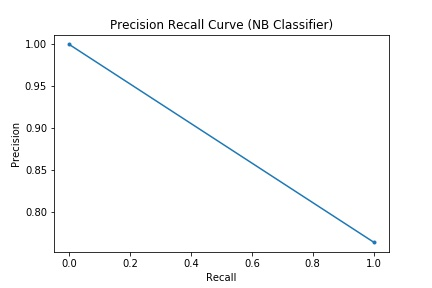
\includegraphics[scale=0.29]{Figures/PRN.jpg}}%
\hfill % <-- Seperation
\subcaptionbox{ROC}{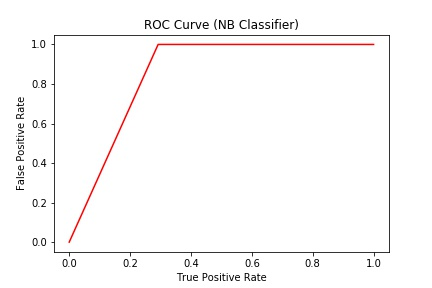
\includegraphics[scale =0.29]{Figures/ROCN.jpg}}%
\caption{Result of Naive Bayes Classifier}
\label{prrn}
\end{figure}

\begin{figure}[H]
\centering
\subcaptionbox{precision-recall}{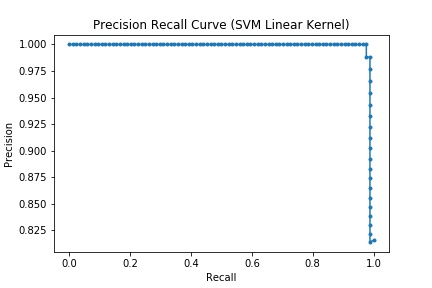
\includegraphics[scale=0.29]{Figures/PRSL.jpg}}%
\hfill % <-- Seperation
\subcaptionbox{ROC}{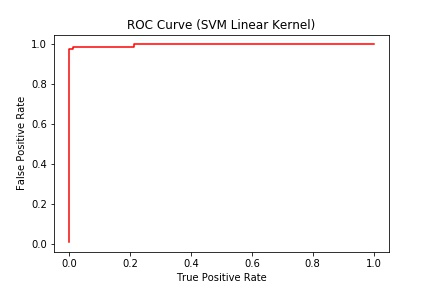
\includegraphics[scale =0.29]{Figures/ROCSL.jpg}}%
\caption{Result of SVM (Linear Kernel)}
\label{slk}
\end{figure}

\begin{figure}[H]
\centering
\subcaptionbox{precision-recall}{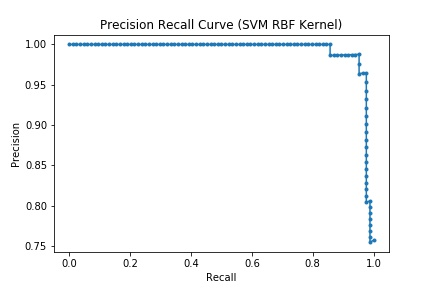
\includegraphics[scale=0.29]{Figures/PRSR.jpg}}%
\hfill % <-- Seperation
\subcaptionbox{ROC}{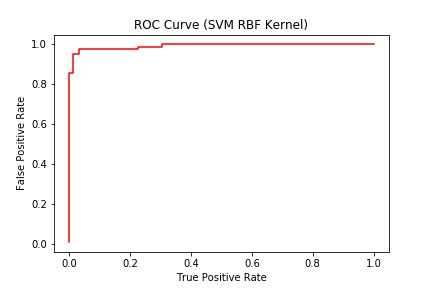
\includegraphics[scale =0.29]{Figures/ROCSR.jpg}}%
\caption{Result of SVM (RBF Kernel)}
\label{svr}
\end{figure}

\begin{figure}[H]
\centering
\subcaptionbox{precision-recall}{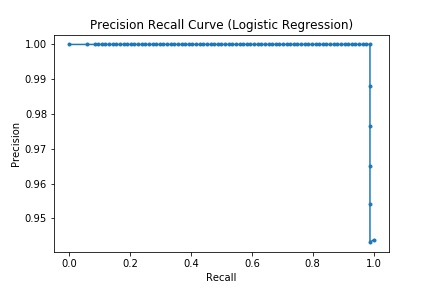
\includegraphics[scale=0.29]{Figures/PRLR.jpg}}%
\hfill % <-- Seperation
\subcaptionbox{ROC}{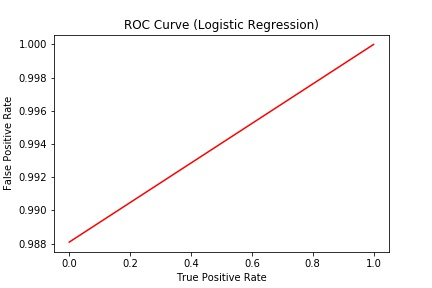
\includegraphics[scale =0.29]{Figures/ROCLR.jpg}}%
\caption{Result of Logistic Regression}
\label{flr}
\end{figure}

\begin{figure}[H]
\centering
\subcaptionbox{precision-recall}{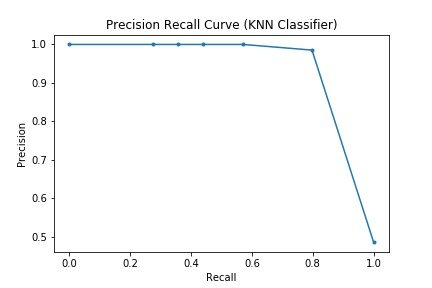
\includegraphics[scale=0.29]{Figures/PRKNN.jpg}}%
\hfill % <-- Seperation
\subcaptionbox{ROC}{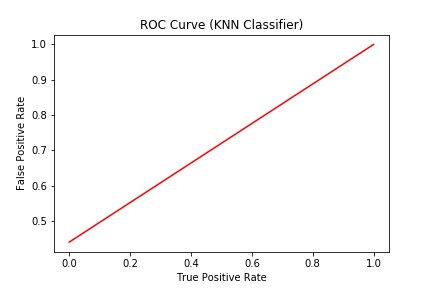
\includegraphics[scale =0.29]{Figures/ROCKNN.jpg}}%
\caption{Result of K-Nearest Neighbor}
\label{fknn}
\end{figure}

\begin{figure}[H]
\centering
\subcaptionbox{precision-recall}{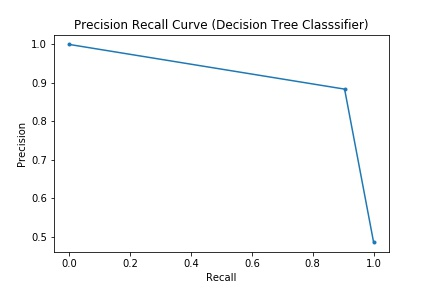
\includegraphics[scale=0.29]{Figures/PRDCT.jpg}}%
\hfill % <-- Seperation
\subcaptionbox{ROC}{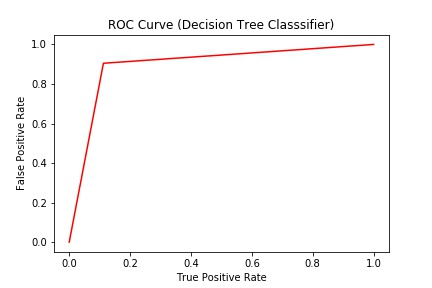
\includegraphics[scale =0.29]{Figures/ROCDCT.jpg}}%
\caption{Result of Decision Tree}
\label{fdct}
\end{figure}

\textbf{Fig.} \ref{fig:out} shows sample input and corresponding output in our system.
\begin{figure}[h!]
\centering
  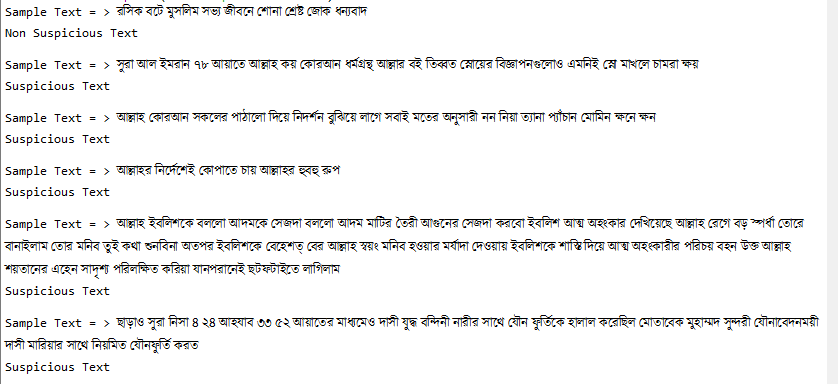
\includegraphics[height=6.8cm, width=8.8cm]{Figures/output.PNG}
  \caption{ Output in System Environment}
  \label{fig:out}
\end{figure}

%%%% Conclusion and Future Improvement %%%%
%%%%%%%%%%%%%%%%%%%%%%%%%%%%%%%%%%%%%%%%%%%
\section{\textbf{Conclusion and Future Improvement}}
In this paper, we have presented suspicious Bangla text detection strategies using different machine learning models, evaluate them and show a comparison of accuracy between this models. We get maximum accuracy of 92$\%$ using Logistic Regression. Support Vector Machine and other algorithms also get mentionable accuracy on our dataset. The overall accuracy of all algorithm can be increased by removing more stop words and by increasing size of the dataset.\par
In future, we plan to use deep learning approach to find semantic relation between words of a text which will help us to predict more accurately. We are planing to construct larger dataset to increase accuracy, efficiency and reliability of our system.


\renewcommand{\bibfont}{\normalfont\small}
\printbibliography

\end{document}


